% This is text associated with the open textbook "Open Electromagnetics"
% See immediately below for author, date
% This work is licensed under the Creative Commons Attribution-ShareAlike 4.0 International License. (CC BY-SA 4.0) 
% To view a copy of the license, visit http://creativecommons.org/licenses/by-sa/4.0/

%ORB TITLE Equivalent Circuit Model for Transmission; Radiation Efficiency
%ORB AUTHOR 0        # S.W. Ellingson, Virginia Tech (ellingson@vt.edu)
%ORB DATE 20191127   # yyyymmdd
%ORB ABSTRACT 

\label{m0202_Equivalent_Circuit_Model_for_Transmission} % <-- Must match name of this file and module directory name.  Don't mess with this!

A radio transmitter consists of a source which generates the electrical signal intended for transmission, and an antenna which converts this signal into a propagating electromagnetic wave.  Since the transmitter is an electrical system, it is useful to be able to model the antenna as an equivalent circuit. 
From a circuit analysis point of view, it should be possible to describe the antenna as a passive one-port circuit that presents an impedance to the source.
Thus, we have the following question: What is the equivalent circuit for an antenna which is transmitting?

We begin by emphasizing that the antenna is passive.  
That is, the antenna does not add power.
Invoking the principle of conservation of power, there are only three possible things that \emph{can} happen to power that is delivered to the antenna by the transmitter:\footnote{Note that ``delivered'' power means power accepted by the antenna. We are not yet considering power reflected from the antenna due to impedance mismatch.}
%
\begin{itemize}
\item Power can be converted to a propagating electromagnetic wave. (The desired outcome.)
\item Power can be dissipated within the antenna.
\item Energy can be stored by the antenna, analogous to the storage of energy in a capacitor or inductor.
\end{itemize}
%
We also note that these outcomes can occur in any combination.
Taking this into account, we model the antenna using the equivalent circuit shown in Figure~\ref{m0202_fAntTxEqCirc}.
%
\begin{figure}[b!] % <--- "[b!]" for first figure in section *only*; delete for 2nd and subsequent figures
\begin{center}
\pdftooltip{{  % note double braces
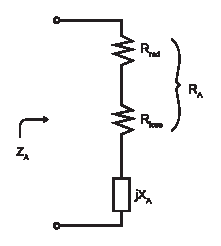
\includegraphics[width=2in]{modules/m0202_AntennaEquivCircuitTransmission.eps} 
% https://commons.wikimedia.org/wiki/File:Transmitting_Antenna_Circuit.svg
}}{An open circuit with capital Z subscript capital A. In series from top to bottom, a resistor (capital R subscript rad), a resistor (capital R subscript loss), and a rectangle labeled small j capital X subscript capital A. The two resistors together are labeled capital R sub capital A. }
\end{center}
\centerline{\scriptsize 
\copyright~\hyperref[m0202_fAntTxEqCirc_Credit]{S.\ Lally} 
\href{https://creativecommons.org/licenses/by-sa/4.0/}{CC BY-SA 4.0} 
} % \centerline 
\caption{
\label{m0202_fAntTxEqCirc}
Equivalent circuit for an antenna which is transmitting.
}
\end{figure}
%
Since the antenna is passive, it is reasonable to describe it as an impedance $Z_A$ which is (by definition) the ratio of voltage $\widetilde{V}_A$ to current $\widetilde{I}_A$ at the terminals; i.e.,
%
\begin{equation}
Z_A \triangleq \frac{\widetilde{V}_A}{\widetilde{I}_A}
\end{equation}
%
In the phasor domain, $Z_A$ is a complex-valued quantity and therefore has, in general, a real-valued component and an imaginary component.  
We may identify those components using the power conservation argument made previously: 
Since the real-valued component must represent power transfer and the imaginary component must represent energy storage, we infer:
%
\begin{equation}
Z_A \triangleq R_A +jX_A
\end{equation}
%
where $R_A$ represents power transferred to the antenna, and $X_A$ represents energy stored by the antenna.  
Note that the energy stored by the antenna is being addressed in precisely the same manner that we address energy storage in a capacitor or an inductor; in all cases, as reactance.
Further, we note that $R_A$ consists of components $R_{rad}$ and $R_{loss}$ as follows:
%
\begin{equation}
Z_A = R_{rad} + R_{loss} +jX_A
\end{equation}
%
where $R_{rad}$ represents power transferred to the antenna and subsequently radiated, and $R_{loss}$ represents power transferred to the antenna and subsequently dissipated. 

To confirm that this model works as expected, consider what happens when a voltage is applied across the antenna terminals.
The current $\widetilde{I}_A$ flows and the time-average power $P_A$ transferred to the antenna is 
%
\begin{equation}
P_A = \frac{1}{2}\mbox{Re}\left\{ \widetilde{V}_A \widetilde{I}^*_A \right\}
\end{equation}
%
where we have assumed peak (as opposed to root mean squared) units for voltage and current.
Since $\widetilde{V}_A = Z_A \widetilde{I}_A$, we have:
%
\begin{equation}
P_A = \frac{1}{2}\mbox{Re}\left\{ \left( R_{rad} + R_{loss} +jX_A \right) \widetilde{I}_A  \widetilde{I}^*_A \right\}
\end{equation}
%
which reduces to:
%
\begin{equation}
P_A = \frac{1}{2}\left|\widetilde{I}_A\right|^2 R_{rad} + \frac{1}{2}\left|\widetilde{I}_A\right|^2 R_{loss}
\label{m0202_ePA}
\end{equation}
%
As expected, the power transferred to the antenna is the sum of 
%
\begin{equation}
P_{rad} \triangleq \frac{1}{2}\left|\widetilde{I}_A\right|^2 R_{rad} 
\label{m0202_ePrad}
\end{equation}
%
representing power transferred to the radiating electromagnetic field, and
%
\begin{equation}
P_{loss} \triangleq \frac{1}{2}\left|\widetilde{I}_A\right|^2 R_{loss} 
\label{m0202_ePloss}
\end{equation}
%
representing power dissipated within the antenna.

The reactance $X_A$ will play a role in determining $\widetilde{I}_A$ given $\widetilde{V}_A$ (and vice versa), but does not by itself account for disposition of power.  Again, this is exactly analogous to the role played by inductors and capacitors in a circuit.

The utility of this equivalent circuit formalism is that it allows us to treat the antenna in the same manner as any other component, and thereby facilitates analysis using conventional electric circuit theory and transmission line theory.  
For example: 
Given $Z_A$, 
we know how to specify the output impedance $Z_S$ of the transmitter so as to minimize reflection from the antenna:  We would choose $Z_S=Z_A$, since in this case the voltage reflection coefficient would be
%
\begin{equation}
\Gamma = \frac{Z_A-Z_S}{Z_A+Z_S} = 0
\end{equation}
% 
Alternatively, we might specify $Z_S$ so as to maximize power transfer to the antenna:  We would choose $Z_S=Z_A^*$; i.e., conjugate matching.

In order to take full advantage of this formalism, we require values for $R_{rad}$, $R_{loss}$, and $X_A$.  
These quantities are considered below.

{\bf Radiation resistance.}
\index{radiation resistance}
$R_{rad}$ is referred to as \emph{radiation resistance}.
Equation~\ref{m0202_ePrad} tells us that
%
\begin{equation}
R_{rad} = 2P_{rad}\left|\widetilde{I}_A\right|^{-2}
\label{m0202_ePrad2}
\end{equation}
%
This equation suggests the following procedure:  We apply current $\widetilde{I}_A$ to the antenna terminals, and then determine the total power $P_{rad}$ radiated from the antenna in response.
For an example of this procedure, see Section~\ref{m0207_Total_Power_Radiated_by_an_Electrically-Short_Dipole} (``Total Power Radiated by an Electrically-Short Dipole'').
Given $\widetilde{I}_A$ and $P_{rad}$, one may then use Equation~\ref{m0202_ePrad2} to determine $R_{rad}$.  

{\bf Loss resistance.}
\index{loss resistance}
\emph{Loss resistance} represents the dissipation of power within the antenna, which is usually attributable to loss intrinsic to materials comprising or surrounding the antenna.  
In many cases, antennas are made from good conductors -- metals, in particular -- so that $R_{loss}$ is very low compared to $R_{rad}$.
For such antennas, loss is often so low compared to $R_{rad}$ that $R_{loss}$ may be neglected.
In the case of the electrically-short dipole, $R_{loss}$ is typically very small but $R_{rad}$ is also very small, so both must be considered.
In many other cases, antennas contain materials with substantially greater loss than metal.
For example, a microstrip patch antenna 
\index{antenna!microstrip patch}
implemented on a printed circuit board
\index{printed circuit board (PCB)}
typically has non-negligible $R_{loss}$ because the dielectric material comprising the antenna exhibits significant loss.

{\bf Antenna reactance.}
The reactance term $jX_A$ accounts for energy stored by the antenna.
This may be due to reflections internal to the antenna, or due to energy associated with non-propagating electric and magnetic fields surrounding the antenna.  The presence of significant reactance (i.e., $\left|X_A\right|$ comparable to or greater than $\left|R_A \right|$) complicates efforts to establish the desired impedance match to the source.
For an example, see Section~\ref{m0210_Reactance_of_the_Electrically-Short_Dipole} (``Reactance of the Electrically-Short Dipole'').

{\bf Radiation efficiency.}
\index{radiation efficiency}
When $R_{loss}$ is non-negligible, it is useful to characterize antennas in terms of their \emph{radiation efficiency} $e_{rad}$, defined as the fraction of power which is radiated compared to the total power delivered to the antenna; i.e.,
%
\begin{equation}
e_{rad} \triangleq \frac{P_{rad}}{P_A}
\end{equation}
%
Using Equations~\ref{m0202_ePA}--\ref{m0202_ePloss}, we see that this efficiency can be expressed as follows:
%
\begin{equation}
e_{rad} = \frac{R_{rad}}{R_{rad}+R_{loss}}
\label{m0202_eRE}
\end{equation}
%
Once again, the equivalent circuit formalism proves useful.

%%%%%%%%%%%%%%%%%%%%%%%%%%%%%%%%%%%%%%%%%%%%%%%
%ORB EXAMPLE
~\\ \begin{example} 
\begin{mdframed}[backgroundcolor=brown!20,linecolor=brown!20]\raggedright
Impedance of an antenna. 
\\~\\
The total power radiated by an antenna is 60~mW when 20~mA (rms) is applied to the antenna terminals.  
The radiation efficiency of the antenna is known to be 70\%.
It is observed that voltage and current are in-phase at the antenna terminals.
Determine (a) the radiation resistance, (b) the loss resistance, and (c) the impedance of the antenna.

{\bf Solution}.
From the problem statement, $P_{rad}=60$~mW, $\left|\widetilde{I}_A\right|=20$~mA (rms), and $e_{rad}=0.7$.
Also, the fact that voltage and current are in-phase at the antenna terminals indicates that $X_A=0$.
From Equation~\ref{m0202_ePrad2}, the radiation resistance is
%
\begin{equation}
R_{rad} \approx \frac{2\cdot\left(60~\mbox{mW}\right)}{\left|\sqrt{2}\cdot 20~\mbox{mA}\right|^2} = \underline{150~\Omega}
\end{equation}
%
Solving Equation~\ref{m0202_eRE} for the loss resistance, we find:
%
\begin{equation}
R_{loss} = \frac{1-e_{rad}}{e_{rad}}R_{rad} \cong \underline{64.3~\Omega}
\end{equation}
%
Since $Z_A=R_{rad}+R_{loss}+jX_A$, we find $Z_A\cong$ \underline{$214.3+j0~\Omega$}.
This will be the ratio of voltage to current at the antenna terminals regardless of the source current.
\end{mdframed}
% note figures will need to go between "\end{mdframed}" and "\end{example}"
\end{example}
%%%%%%%%%%%%%%%%%%%%%%%%%%%%%%%%%%%%%%%%%%%%%%%

